%\input{sections/martian-environment/references.tex}



\section{Dust}
\label{sec:MartianEnvironment:Dust}
%\input{sections/s.tex}

% Martian Season - start with images
% Regolith, dust, and craters, other elements
% Settle with locations DTMS

The red planet's axis is tilted away from the sun at \si{25}{\degree}. Very much like Earth's \si{23.5}{\degree} axial tilt, this results in seasons. Mars has an orbit with a semi-major axis of \si{1.524}{\astronomicalunit} which translantes to a MArtian year corresponding to an orbital period of 687 days. Martian seasons are longer and for every Martian year 1.88 Earth years go by. Sidereal days are 24.62 hours long and solar days are 24.65 hours long. A Martian day, known as a Sol, is approximately 40 minutes longer than an Earth day.

The apparent seasonal advance of the Sun at Mars is commonly measured in terms of the areocentric longitude Ls, as referred to the planet's vernal equinox (the ascending node of the apparent seasonal motion of the Sun on the planet's equator). The relationship betweeen the areocentric longitude, Sol, and Martian day with respect to the planet's seasonal advances are presented in Table \ref{table:mars-seasonal-advances}

\begin{table}[H]
  \centering
  \caption{Seasonal advances on Mars.}
  \label{tab:mars-seasonal-advances}
  \begin{tabular}{|l|l|l|}
  \hline
  \multirow{2}{*}{\textbf{\begin{tabular}[c]{@{}l@{}}Areocentric\\ Longitude\end{tabular}}} & \multicolumn{2}{c|}{\textbf{Seasonal Advance}} \\ \cline{2-3}
   & \multicolumn{1}{c|}{\textbf{Northern Hemisphere}} & \multicolumn{1}{c|}{\textbf{Southern Hemisphere}} \\ \hline
  \textbf{\si{0}{\degree}} & Vernal Equinox & Autumnal Equinox \\ \hline
  \textbf{\si{0}{\degree} to \si{90}{\degree}} & Spring & Autumn \\ \hline
  \textbf{\si{90}{\degree}} & Summer Solstice & Winter Solstice \\ \hline
  \textbf{\si{90}{\degree} to \si{180}{\degree}} & Summer & Winter \\ \hline
  \textbf{\si{180}{\degree}} & Autumnal Equinox & Vernal Equinox \\ \hline
  \textbf{\si{180}{\degree} to \si{270}{\degree}} & Autumn & Spring \\ \hline
  \textbf{\si{270}{\degree}} & Winter Solstice & Summer Solstice \\ \hline
  \textbf{\si{270}{\degree} to \si{360}{\degree}} & Winter & Summer \\ \hline
  \end{tabular}
\end{table}


Areocentric longitude values of \si{0}{\degree}, \si{90}{\degree}, \si{180}{\degree}, and \si{270}{\degree}


 indicate the vernal equinox, summer solstice, autumnal equinox, and winter solstice, respectively.


\si{kg.m.s^{-1}}

 The great fluctuations in temperature and the difference in warmth between hemispheres can cause huge dust storms. Some can affect just a small area, while others can cover the entire planet. The larger storms usually occur when the planet is near its aphelion(closest point to the Sun). When there are global dust storms there is no way for scientists to visualize the planet’s surface.

\begin{figure}[H]%[b]
%\vspace{-2ex}
  \centering
  \hypersetup{linkcolor=captionTextColor}
  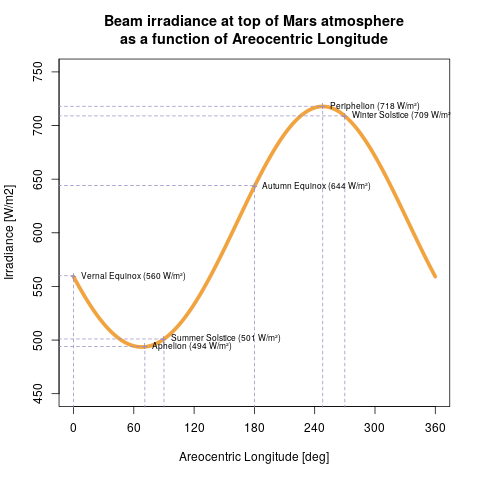
\includegraphics[width=0.8\linewidth]{sections/martian-environment/plots/beam-irradiance-at-top-of-mars-atmosphere-as-a-function-of-areocentric-longitude.png}\\
  %\vspace{-2ex}
  \caption[Beam irradiance at top of Mars atmosphere as a function of Areocentric Longitude]
          {Beam irradiance at top of Mars atmosphere as a function of Areocentric Longitude}
  \label{fig:plot:beam-irradiance-top-of-mars-atmosphere}
  %\vspace{-3ex}
\end{figure}

Great dust storms (area > 10e6 km2) occur with a yearly probability of 30\% to 80\%. \citepower{Kerslake1999}

Local dust storms (area < 10e6 km2) occur with a 5\% probability in Mars equatorial regions and have only a minor impact on seasonal insulation due to their limited size, duration (a few days), and moderate OD (~1). \citepower{Kerslake1999}

the dust accumulation rate is assumed to be 5\% of that measured by Pathfinder \citepower{Kerslake1999}

Losses from lander vehicle shadowing and terrain masking are not yet modeled pending better definitions of lander configuration and landing sites. \citepower{Kerslake1999}

For desirable near-equatorial landing sites (not in canyons), shadowing and terrain masking losses will be small. This is due to high sun angles (that create short shadows) and the large component of diffuse solar insolation near dusk and dawn (when the terrain masking effect is largest). \citepower{Kerslake1999}


\section{Dust Storms}
\label{sec:MartianEnvironment:DustStorms}
%\input{sections/s.tex}
